\section{Preliminaries}
\label{sec:prelim}

Let $I$ be a bag of $N$ closed-open time intervals from time domain
$T$ representing validity periods of tuples in some relation $R$:

$I = [\![ ~[s,e) ~|~ s < e ]\!]$

Intervals in $I$ may be overlapping, duplicates of each other, etc.

The objective is to partition $I$ among machines in a cluster to
achieve load balancing.  For load balancing we want to place
approximately equal number of intervals in each partition.  This cost
model is based on the assumption that the target cluster is
homogeneous and time locality is required.  For example, temporal
aggregation $\theta^T$ requires such locality to compute aggregates at
each time instant and its performance is a function of the size of the
partition.  Following Le et al.~\cite{Le2013} who proposed the
sequential algorithm for this problem, we define the cost of the
partition $P$ over $I$ of size $k$ as follows:

\begin{itemize}
\item $P$ contains $k$ distinct time instances/lines called {\em
  splitters} that divide the overall time of $I$ into $k+1$ buckets:
  $P = l_1,\ldots,l_k$, $l \in \mathbb{T}$.  We assign $l_0 = -\infty$
  and $l_{k+1} = \infty$ and define buckets as time periods between
  splitters: $b_i = [l_{i-1}, l_i), 1 \leq i \leq k+1$.

\item An interval is assigned to a bucket if it intersects with it,
  i.e. $b_i = [\![ ~[s,e) \in I ~|~ [s,e) \cap [l_{i-1},l_i) \neq
            \emptyset ]\!]$.  Each interval of $I$ may be assigned to
        more than one bucket if it is not wholly contained in one.
        The size of the bucket is the total number of intervals
        assigned to it.  Observe that the total number of intervals in
        the partition can be, and usually is, larger than N:
        $\sum_{i=1}^{k+1} |b_i| \geq N$.

\item Since the time of the distributed computation is determined by
  the stragglers, we define the cost of the partition as the size of
  the largest bucket: $c(P) = max\{|b_1|,\ldots,|b_{k+1}|\}$.

\end{itemize}

The optimal partition of size $k$ over $I$ is a partition with the
lowest cost:

$P^*(k,I) = argmin~ c(P)$, where $P \in \mathbf{P}(I,k)$ and
$\mathbf{P}$ is the set of all possible partitions of $I$ of size {\em
  up to} $k$.

\begin{figure}
\centering
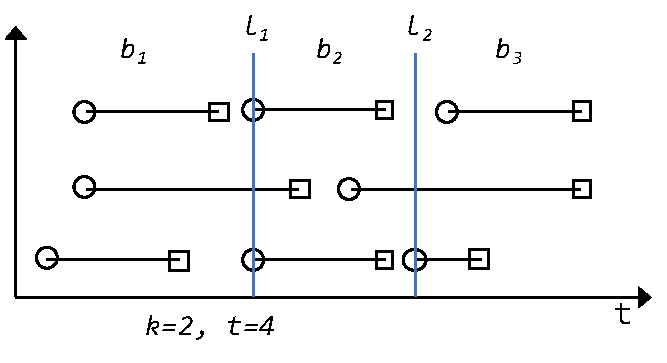
\includegraphics[width=2.5in]{figs/buckets.pdf}
\caption{Example optimal partition.}
\label{fig:example}
\end{figure}

As an illustration, consider Figure~\ref{fig:example}.  $I$ consists
of 8 intervals. An optimal partition of size 2 with cost 4 is shown.
As Le proved in~\ref{Le2013}, we need only consider interval start
times as candidate splitters.  Splitting on any other times in the
lifespan of $I$ produces partitions that are no more optimal, and
generally less optimal.  Observe that a partition with lower cost of
the same size is not feasible.

We are interested in an efficient {\em distributed} solution for
finding $P^*$ for cases of very large $I$.
